\listfiles
\documentclass[final,5p,times,twocolumn]{elsarticle}
\usepackage{adjustbox}
\usepackage{algorithm,algorithmic}
\usepackage{amsfonts}
\usepackage{amsmath,amssymb}
\usepackage{booktabs}
\usepackage{color,colortbl}
\usepackage{comment}
\usepackage{float}
\usepackage{graphicx}
\usepackage{subcaption} 
\usepackage{mathrsfs}
\usepackage{multirow}
\usepackage{hyperref}
\usepackage{tikz}
\usepackage{svg}
\usepackage{threeparttable}
\usepackage[spanish,es-tabla,es-lcroman]{babel}
\usepackage{pgfplots}
\pgfplotsset{compat=1.5}
\usepgfplotslibrary{external}
\tikzexternalize

\hypersetup{
 colorlinks=true,
 linkcolor=black,
 urlcolor=black,
 filecolor=black,      
 pdfpagemode=FullScreen,
}
\pdfstringdefDisableCommands{%
  \def\corref#1{}%
}

\bibliographystyle{IEEEtran}

\begin{document}

\begin{frontmatter}

\title{Optimización del problema de localización de microhubs y asignación peatonal (TMLPA) utilizando el Algoritmo de la Morsa Binario}


\author[uv]{Jorge Quiroz Hernández\corref{cor}}

\address[uv]{Escuela de Ingeniería Informática, Universidad de Valparaíso, Chile.}
\cortext[cor]{Corresponding author}\ead{jorge.quirozh@postgrado.uv.cl}

\begin{abstract}
La logística de transporte urbano de carga enfrenta importantes cuellos de botella operativos durante las horas de mayor demanda, lo que exige paradigmas de distribución más flexibles. Este estudio evalúa el Problema de Localización de Microhubs y Asignación Peatonal (TMLPA) con el objetivo de minimizar los costos fijos de instalación, los costos de procesamiento y las distancias de caminata. Se introduce el Algoritmo de la Morsa Binario (BWO) con mecánicas de explotación multimodales, evaluando su rendimiento frente a una línea base de Optimización por Enjambre de Partículas Binario (BPSO) y los límites exactos de Programación Lineal Entera Mixta (MILP) resueltos mediante el motor HiGHS. A lo largo de 30 ejecuciones independientes, se identificaron los valores atípicos mediante filtros estadísticos y se reemplazaron en tiempo real para garantizar la integridad de las muestras. En escalas pequeñas (3 puntos de entrega, 5 clientes), ambas metaheurísticas alcanzaron una precisión del $100\%$, igualando el óptimo global exacto de $84,2000$. En matrices medianas (10 puntos de entrega, 25 clientes), BPSO convergió prematuramente a un pozo local de $461,0000$ ($+1,99\%$ de brecha) debido a una pérdida total de diversidad, mientras que BWO preservó la varianza exploratoria, alcanzando un mejor valor de $464,8000$ ($+2,83\%$ de brecha). En la escala más grande (20 puntos de entrega, 50 clientes), BPSO logró acercarse al límite global ($915,2000$) con un costo mínimo de $920,3000$ ($+0,56\%$ de brecha), mientras que BWO equilibró un rango de búsqueda más amplio alcanzando los $933,1000$ ($+1,96\%$ de brecha). Las pruebas no paramétricas de Mann-Whitney-Wilcoxon confirmaron diferencias significativas en la distribución ($p < 0,0001$) en escalas medianas y grandes, mapeando los límites explícitos para el despliegue de heurísticas en topografías de asignación no lineales.
\end{abstract}

\begin{keyword}
Logística de última milla \sep Localización y asignación de microhubs \sep Algoritmo de la morsa binario \sep Optimización por enjambre de partículas \sep Estadística no paramétrica \sep Verificación de límites exactos
\end{keyword}

\end{frontmatter}

\section{Introducción}
\label{sec:introduction}
El crecimiento exponencial del comercio electrónico ha generado una presión significativa sobre la infraestructura de distribución de última milla en entornos metropolitanos. Los envíos directos al consumidor provocan un incremento en la congestión vehicular, las emisiones de carbono y la complejidad de la planificación de rutas de entrega. Para mitigar estos impactos urbanos, los puntos de entrega \textit{microhubs} temporales han emergido como una alternativa descentralizada y eficiente. Estos puntos funcionan como centros de consolidación local donde los paquetes se agrupan, lo que permite a los transportistas realizar entregas en lotes y transferir el tramo final del trayecto al consumidor.

La optimización de estos sistemas requiere resolver dos subproblemas de manera simultánea: determinar qué puntos de entrega potenciales deben habilitarse a partir de un conjunto finito de espacios disponibles y asignar los usuarios a los nodos activos, respetando las restricciones operacionales. Este desafío se denomina Problema de Localización de Microhubs y Asignación Peatonal (TMLPA) \textit{(Two-Echelon Microhub Location-Allocation Problem)}. El objetivo principal consiste en minimizar una función de costo global no lineal que integra los costos fijos de habilitación, las tarifas de procesamiento dependientes de la demanda y las penalizaciones por insatisfacción del cliente ponderadas por su nivel de prioridad.

A pesar de que los enfoques matemáticos deterministas, como la programación lineal entera mixta (MILP, por sus siglas en inglés), aseguran la obtención de óptimos globales en instancias acotadas, sus tiempos de cómputo escalan de forma exponencial respecto al número de puntos de entrega y clientes candidatos. Este cuello de botella computacional invalida su uso para la toma de decisiones en tiempo real o para la planificación en escenarios urbanos de gran escala. Por consiguiente, las metaheurísticas de enjambre bioinspiradas se han consolidado como la estrategia predominante para explorar eficientemente estos espacios de búsqueda no lineales \cite{Shami2022}.

Este estudio implementa un marco de evaluación competitivo para resolver este desafío y sus principales contribuciones son:

\begin{enumerate}
    \item Se introduce una formulación binaria del Algoritmo de Optimización de la Morsa \textit{(Binary Walrus Optimizer, BWO)}~\cite{han2023walrus} para resolver las restricciones de localización y asignación peatonal del TMLPA.
    \item Se realizan pruebas de rendimiento comparativas frente a una implementación de referencia de Optimización por Enjambre de Partículas Binario (BPSO) sobre tres escalas de magnitud distintas ($3 \times 5$, $10 \times 25$ y $20 \times 50$).
    \item Se establecen métricas de verdad absoluta empírica para todas las evaluaciones, utilizando el motor de optimización MILP HiGHS integrado en la plataforma MiniZinc~\cite{nethercote2007minizinc}.
    \item Se aplican filtros de control de calidad estadístico explícitos durante la recolección de datos ($N=30$), identificando, eliminando y reejecutando dinámicamente los valores atípicos para preservar el tamaño de la muestra y la validez de las inferencias no paramétricas posteriores. 
\end{enumerate}

El resto de este artículo se organiza de la siguiente manera: la Sección~\ref{sec:mathematical_model} formaliza el modelo matemático del TMLPA. La Sección~\ref{sec:metaheuristic_frameworks} detalla las adaptaciones discretas de los modelos BPSO y BWO, mientras que la Sección~\ref{sec:experimental_setup} describe los parámetros experimentales y el protocolo de manejo de valores atípicos. Por su parte, la Sección~\ref{sec:results} presenta las métricas cuantitativas, valoraciones estadísticas y análisis de convergencia. Finalmente, la Sección~\ref{sec:discussion} analiza las compensaciones conductuales entre exploración y explotación antes de concluir en la Sección~\ref{sec:conclusion}.

\section{Formulación del Modelo Matemático}
\label{sec:mathematical_model}
El TMLPA se modela sobre una topografía de optimización constituida por un conjunto discreto de clientes a pie $C = \{1, 2, \dots, n\}$ y un conjunto de potenciales puntos de entrega temporales (microhubs) $J = \{1, 2, \dots, m\}$. Cada cliente $c \in C$ presenta un volumen escalar fijo de demanda logística $q_c$ y una ponderación de prioridad de servicio asociada $w_c > 0$. Las distancias espaciales entre las entidades se definen mediante una matriz estática $d_{cj}$, la cual representa la distancia a pie desde el cliente $c$ hasta el punto de entrega candidato $j$. 

Cada punto de entrega candidato $j \in J$ está restringido por una capacidad volumétrica límite $L_j$, un costo fijo de habilitación $f_j$ y un factor de costo variable $o_j$. Este último correspondiente al costo operacional por cada unidad de demanda procesada. La distancia máxima permisible para el tránsito a pie de los usuarios está acotada por un umbral global $D_{\max}$. Adicionalmente, el sistema aplica un límite estricto de presupuesto operativo, exigiendo que el número total de puntos habilitados se encuentre dentro del intervalo $[P_{\min}, P]$.

Sea $y_j \in \{0, 1\}$ la variable de decisión binaria que indica si el punto de entrega $j$ está activo ($y_j = 1$) o permanece cerrado ($y_j = 0$). Asimismo, la variable $x_{cj} \in \{0, 1\}$ corresponde al parámetro de asignación, indicando si el cliente $c$ está asociado al punto $j$ ($x_{cj} = 1$) o no ($x_{cj} = 0$). Con estas definiciones, el marco de optimización matemática se estructura de la siguiente manera:

\begin{equation}
\min_{x, y} Z = \sum_{j \in J} f_j y_j + \sum_{j \in J} \sum_{c \in C} o_j q_c x_{cj} + \sum_{c \in C} \sum_{j \in J} w_c d_{cj} x_{cj}
\label{eq:objective}
\end{equation}

Sujeto a las siguientes restricciones del sistema:
\begin{align}
\sum_{j \in J} x_{cj} &= 1, \quad \forall c \in C \label{ctx:single_assignment} \\
x_{cj} &\le y_j, \quad \forall c \in C, \, \forall j \in J \label{ctx:activation_gate} \\
\sum_{c \in C} q_c x_{cj} &\le L_j y_j, \quad \forall j \in J \label{ctx:capacity} \\
d_{cj} x_{cj} &\le D_{\max}, \quad \forall c \in C, \, \forall j \in J \label{ctx:distance} \\
P_{\min} \le \sum_{j \in J} y_j &\le P \label{ctx:hub_bounds} \\
x_{cj}, y_j &\in \{0, 1\}, \quad \forall c \in C, \, \forall j \in J \label{ctx:binary}
\end{align}

La ecuación~\eqref{eq:objective} define la función objetivo global, la cual minimiza tres componentes: los costos fijos de activación totales, los costos variables de procesamiento de la demanda y las distancias de caminata de los clientes hacia los puntos de entrega, escaladas por su respectiva ponderación de prioridad de servicio.
La restricción~\eqref{ctx:single_assignment} asegura que cada cliente sea asignado a exactamente un punto de entrega.
Por su parte, la restricción~\eqref{ctx:activation_gate} actúa como una compuerta de activación, forzando que un cliente solo pueda asociarse a un punto de entrega si dicho nodo ha sido seleccionado para su habilitación. 

La restricción~\eqref{ctx:capacity} previene que la demanda acumulada asignada a un punto de entrega exceda su límite de capacidad volumétrica $L_j$. Asimismo, la restricción~\eqref{ctx:distance} garantiza que se cumplan los límites de accesibilidad espacial $D_{\max}$ para resguardar la comodidad del cliente. A su vez, la restricción~\eqref{ctx:hub_bounds} acota el número total de puntos de entrega abiertos dentro de los umbrales de presupuesto operativos $[P_{\min}, P]$, mientras que la restricción~\eqref{ctx:binary} delimita el espacio de soluciones a variables estrictamente binarias.

\section{Marcos Metaheurísticos}
\label{sec:metaheuristic_frameworks}

\subsection{Optimización por Enjambre de Partículas Binario (BPSO)}
Este enfoque de optimización utiliza una formulación discreta modificada del algoritmo estándar de Optimización por Enjambre de Partículas \textit{(Particle Swarm Optimization)}~\cite{Shami2022}. Cada partícula $i$ dentro de un espacio de búsqueda continuo mantiene un registro de su vector de posición actual $x_i$, su mejor posición histórica personal $p_i^*$ y la mejor posición global alcanzada por el enjambre $g^*$. Para mapear las actualizaciones continuas a las variables binarias discretas exigidas por la ecuación~\eqref{ctx:binary}, se aplica una función de transferencia sigmoidea estándar. Las ecuaciones de actualización estructural para la velocidad $v_{i,j}^{t+1}$ y el estado binario $x_{i,j}^{t+1}$ en cada iteración $t$ se calculan como se describe a continuación:

\begin{equation}
v_{i,j}^{t+1} = \theta v_{i,j}^t + \alpha \epsilon_1 \left( g_j^* - x_{i,j}^t \right) + \beta \epsilon_2 \left( p_{i,j}^* - x_{i,j}^t \right)
\label{eq:bpso_velocity}
\end{equation}

\begin{equation}
S\left( v_{i,j}^{t+1} \right) = \frac{1}{1 + \exp\left( -v_{i,j}^{t+1} \right)}
\label{eq:bpso_sigmoid}
\end{equation}

\begin{equation}
x_{i,j}^{t+1} = \begin{cases} 
1, & \text{si } r_{i,j} < S\left( v_{i,j}^{t+1} \right) \\ 
0, & \text{en caso contrario} 
\end{cases}
\label{eq:bpso_position}
\end{equation}

donde $\theta = 0.7$ representa el coeficiente estático de inercia, $\alpha = 1.7$ y $\beta = 1.7$ corresponden a los coeficientes de aceleración cognitiva y social, respectivamente, mientras que $\epsilon_1, \epsilon_2, r_{i,j} \sim \mathcal{U}(0, 1)$ representan variables aleatorias independientes uniformemente distribuidas.

\subsection{Algoritmo de Optimización Binario de la Morsa (BWO)}
El Algoritmo de Optimización Binario de la Morsa \textit{(Binary Walrus Optimizer)} imita los comportamientos biológicos de las poblaciones de morsas, los cuales incluyen procesos de migración, conductas de protección social y maniobras de combate agresivas~\cite{han2023walrus}. Sea $X_{i,j}^t$ la posición multidimensional de búsqueda del agente $i$ durante la iteración $t$. Las actualizaciones de posición son reguladas por tres estados conductuales primarios, los cuales son dictados por un factor de balance adaptativo $\beta_t$:

\begin{equation}
X_{i,j}^{t+1} = \begin{cases}
X_{i,j}^t + \alpha \cdot (X_{\text{target},j} - X_{i,j}^t), & \text{Migración} \\
X_{i,j}^t + \beta_t \cdot \gamma \cdot (X_{\text{best},j} - X_{i,j}^t), & \text{Protección} \\
X_{i,j}^t - \delta \cdot |X_{\text{combat},j} - X_{i,j}^t|, & \text{Combate}
\end{cases}
\label{eq:bwo_continuous}
\end{equation}

Para cumplir con las exigencias discretas de las restricciones de asignación y habilitación del TMLPA, los vectores de posición continuos se mapean a un dominio binario utilizando una función de transferencia de tangente hiperbólica:

\begin{equation}
T\left( X_{i,j}^{t+1} \right) = \left| \tanh\left( X_{i,j}^{t+1} \right) \right|
\label{eq:bwo_tanh}
\end{equation}

\begin{equation}
X_{\text{binario}, i,j}^{t+1} = \begin{cases}
1, & \text{si } \rho_{i,j} < T\left( X_{i,j}^{t+1} \right) \\
0, & \text{en caso contrario}
\end{cases}
\label{eq:bwo_binary}
\end{equation}
donde $\rho_{i,j} \sim \mathcal{U}(0, 1)$ actúa como un parámetro de umbral para la exploración estocástica.

\subsection{Motor de Aplicación de Restricciones}
Para garantizar la factibilidad estructural respecto a las restricciones~\eqref{ctx:single_assignment} hasta~\eqref{ctx:distance}, ambos algoritmos interactúan con un módulo automatizado de asignación ávida \textit{greedy allocation)}. Cuando un agente de búsqueda actualiza su vector de posición, modifica directamente el vector de activación de puntos de entrega $y$. Si la configuración de puntos de entrega activos infringe los límites de presupuesto operativo $[P_{\min}, P]$, una heurística de reparación modifica aleatoriamente los bits de activación hasta que el vector sea válido.

Una vez que se establece un vector de activación válido $y$, cada cliente $c \in C$ se asigna a su punto de entrega activo más cercano que cumpla simultáneamente con el límite de distancia máxima $D_{\max}$ y con la restricción de capacidad $L_j$. Si un cliente determinado no puede ser asignado de manera factible debido a restricciones de capacidad o distancia, el vector completo de configuración de puntos de entrega $y$ se penaliza mediante un multiplicador de costo prohibitivo ($10^6$). Esto fuerza al enjambre a descartar regiones de búsqueda infactibles.

\section{Configuración Experimental}
\label{sec:experimental_setup}
El desempeño empírico de ambas metaheurísticas se evaluó utilizando tres instancias de prueba, las cuales representan diferentes escalas de distribución urbana:
\begin{itemize}
    \item \textbf{Escala Pequeña} (\texttt{instance\_small.dzn}): $3$ puntos de entrega $\times$ $5$ clientes.
    \item \textbf{Escala Mediana} (\texttt{instance\_medium.dzn}): $10$ puntos de entrega $\times$ $25$ clientes.
    \item \textbf{Escala Grande} (\texttt{instance\_large.dzn}): $20$ puntos de entrega $\times$ $50$ clientes.
\end{itemize}

Para aislar la naturaleza estocástica de las metaheurísticas, cada algoritmo se ejecutó en $30$ ejecuciones independientes utilizando semillas pseudoaleatorias distintas y aisladas que abarcaron el intervalo de enteros $[43, 72]$. El tamaño de la población para cada enjambre se fijó en $30$ agentes, registrando sus trayectorias de convergencia a lo largo de un límite de $100$ iteraciones por cada ejecución independiente.

Con el fin de resguardar la integridad de los datos, se aplicó un filtro dinámico para el manejo de valores atípicos al finalizar cada bloque de simulación. Luego de completar las $30$ ejecuciones de una instancia, se calculó el Rango Intercuartílico (IQR) de los valores de la función objetivo. Cualquier ejecución cuyo resultado se ubicara fuera del intervalo $[Q_1 - 1,5 \times \text{IQR}, Q_3 + 1,5 \times \text{IQR}]$ se clasificó como un valor atípico estadístico \textit{(outlier)}. Estos registros fueron eliminados del conjunto de datos y reejecutados en caliente utilizando una nueva semilla independiente, manteniendo así un tamaño de muestra estable de $N=30$ observaciones válidas para el análisis estadístico posterior.

Los límites globales exactos se certificaron mediante rutinas de cómputo en paralelo empleando el método de ramificación y corte \textit{(branch and cut)} para Programación Lineal Entera Mixta (MILP) a través del motor de optimización HiGHS, integrado en la interfaz de línea de comandos de MiniZinc~\cite{nethercote2007minizinc}. Para optimizar los tiempos de procesamiento, todos los experimentos se desarrollaron en un servidor Dell PowerEdge T140 configurado con un procesador Intel Xeon E-2124 de $3,30$ GHz y $20$ GB de memoria RAM DDR4.

Los códigos fuente del modelo MiniZinc, los scripts de las metaheurísticas y las instancias evaluadas se encuentran disponibles de forma pública en el repositorio de GitHub (\url{https://github.com/jorgequirozh/JQUIROZ-PROYECTO-IAA-MIA-2026}).

\section{Análisis de Resultados Empíricos}
\label{sec:results}

\subsection{Matriz de Rendimiento Cuantitativo}
El resumen estadístico asociado al desempeño de todas las instancias evaluadas se encuentra consolidado en la Tabla~\ref{tab:descriptive_metrics}. Adicionalmente, se determinó la Brecha de Optimización \textit{(Optimality Gap)} calculada como el porcentaje de desviación del mejor valor de la función objetivo alcanzado por cada algoritmo respecto al óptimo global exacto provisto por el motor HiGHS MILP.

\begin{table*}[t]
\centering
\caption{Matriz de Rendimiento Consolidada: Metaheurísticas vs. Límites HiGHS Exactos}
\label{tab:descriptive_metrics}
\small
\begin{threeparttable}
\begin{tabular}{llrrrrrrrrr}
\toprule
\textbf{Instancia} & \textbf{Algoritmo/Motor} & \textbf{Mejor} & \textbf{Peor} & \textbf{$\mu$\tnote{1}} & \textbf{Mediana} & \textbf{$\sigma$\tnote{2}} & \textbf{IQR\tnote{3}} & \textbf{SR\tnote{4}} & \textbf{SS\tnote{5}} & \textbf{Out\tnote{6}} \\
\midrule
\textbf{Pequeña} & Óptimo HiGHS & \textbf{84,2000} & -- & -- & -- & -- & -- & -- & -- & -- \\
($3 \times 5$) & BPSO & 84,2000 & 84,2000 & 84,2000 & 84,2000 & 0,0000 & 0,0000 & 1,0000 & 1,0100 & 0 \\
 & BWO & 84,2000 & 84,2000 & 84,2000 & 84,2000 & 0,0000 & 0,0000 & 1,0000 & 1,0100 & 0 \\
\midrule
\textbf{Mediana} & Óptimo HiGHS & \textbf{452,0000} & -- & -- & -- & -- & -- & -- & -- & -- \\
($10 \times 25$) & BPSO & 461,0000 & 461,0000 & 461,0000 & 461,0000 & 0,0000 & 0,0000 & 0,0000 & 0,0000 & 0 \\
 & BWO & 464,8000 & 473,5000 & 468,9767 & 469,8000 & 2,5127 & 3,2000 & 0,0000 & 0,0000 & 2 \\
\midrule
\textbf{Grande} & Óptimo HiGHS & \textbf{915,2000} & -- & -- & -- & -- & -- & -- & -- & -- \\
($20 \times 50$) & BPSO & 920,3000 & 946,9000 & 930,6000 & 926,2000 & 7,8947 & 11,9750 & 0,0000 & 0,0000 & 0 \\
 & BWO & 933,1000 & 1076,4000 & 1006,1533 & 1003,5000 & 34,2454 & 57,2250 & 0,0000 & 0,0000 & 0 \\
\bottomrule
\end{tabular}

\begin{tablenotes}\footnotesize
    \item[1] \textbf{$\mu$}: Promedio aritmético global de la función objetivo calculado sobre $N=30$ ejecuciones independientes.
    \item[2] \textbf{$\sigma$}: Desviación estándar muestral de la muestra estabilizada.
    \item[3] \textbf{IQR}: Rango intercuartílico utilizado por el filtro de control de calidad estadístico.
    \item[4] \textbf{SR} (\textit{Success Rate}): Tasa de éxito; proporción de corridas que alcanzan el óptimo absoluto.
    \item[5] \textbf{SS} (\textit{Search Speed}): Velocidad de búsqueda expresada mediante convergencia generacional normalizada.
    \item[6] \textbf{Out}: Cantidad de valores atípicos detectados de forma dinámica y reemplazados en caliente.
\end{tablenotes}
\end{threeparttable}
\end{table*}

En la instancia a pequeña escala (\texttt{instance\_small.dzn}), ambos algoritmos demostraron una absoluta estabilidad estructural. El módulo de asignación ávida manejó eficientemente este espacio de búsqueda acotado, permitiendo que ambos enjambres encontraran el óptimo global exacto de $84,2000$ en la totalidad de las simulaciones. Esto se tradujo en tasas de éxito perfectas ($\text{SRate} = 1,0000$), velocidades idénticas ($\text{SSpeed} = 1,0100$) y nula variabilidad ($\sigma = 0,0000$). El vector de activación estructural óptimo encontrado por ambos enfoques coincide con la solución exacta real: $y = [1, 0, 1]$.

Para el problema de escala mediana (\texttt{instance\_medium.dzn}), el mínimo global matemático se estableció en $452,0000$ mediante el método de ramificación y corte de HiGHS, activando la configuración de puntos de entrega $y = [1, 1, 1, 0, 0, 0, 1, 0, 0, 1]$. Ninguna de las metaheurísticas logró alcanzar este óptimo global debido a la presencia de un mínimo local multimodal engañoso ubicado en $461,0000$. El algoritmo BPSO exhibió una convergencia prematura, quedando las $30$ ejecuciones atrapadas de forma unánime en dicha meseta de costo local ($\mu = 461,0000$, $\sigma = 0,0000$), lo que representa una Brecha de Optimización de $+1,99\%$ ($y = [1, 1, 1, 0, 1, 0, 0, 0, 0, 1]$).

En contraste, el Algoritmo de Optimización de la Morsa (BWO) propuesto mantuvo un comportamiento de búsqueda dinámico y exploratorio, evitando el estancamiento prematuro ($\sigma = 2,5127$). Este enfoque alcanzó un mejor valor de la función objetivo de $464,8000$ (Brecha de Optimización de $+2,83\%$) junto con un rendimiento promedio global de $468,9767$. Durante estas ejecuciones de escala mediana, el filtro dinámico de valores atípicos se ejecutó en dos ocasiones, eliminando dos observaciones anómalas \textit{(outliers)} y reemplazándolas en caliente mediante nuevas simulaciones independientes para resguardar la integridad muestral.

En la configuración de mayor escala (\texttt{instance\_large.dzn}), el óptimo global exacto se verificó en $915,2000$, correspondiente a la activación de los puntos de entrega $y = [0, 1, 1, 0, 0, 0, 1, 0, 0, 1, 0, 0, 1, 0, 0, 0, 0, 0, 0, 0]$. El algoritmo base BPSO convergió de manera cercana en torno al óptimo absoluto, logrando un valor mínimo de $920,3000$ y una Brecha de Optimización de apenas $+0,56\%$. Sus ejecuciones se mantuvieron fuertemente agrupadas, lo cual queda evidenciado por una desviación estándar de $7,8947$ y un costo medio de $930,6000$.

Por su parte, el algoritmo BWO propuesto exhibió una dispersión exploratoria significativamente mayor dentro del universo ampliado de esta última instancia ($\sigma = 34,2454$), convergiendo en una mejor solución de $933,1000$ (Brecha de Optimización de $+1,96\%$) y un costo promedio de $1006,1533$. Finalmente, cabe destacar que no se registraron valores atípicos ni se requirieron reemplazos de ejecuciones durante las simulaciones de esta escala mayor.

\subsection{Inferencias No Paramétricas}
Debido a que las soluciones obtenidas por los algoritmos estocásticos no garantizan el cumplimiento de los supuestos de distribución normal, y de acuerdo con la metodología propuesta por Derrac et al. \cite{derrac2011practical}, se aplicó la prueba no paramétrica bilateral de Mann-Whitney-Wilcoxon. Esto permite evaluar la significancia estadística de las diferencias de rendimiento observadas entre BPSO y el algoritmo BWO propuesto. Las métricas estadísticas resultantes para cada escala del problema se resumen en la Tabla~\ref{tab:statistical_inference}.

\begin{table}[h]
\centering
\caption{Métricas de la Prueba de Hipótesis de Mann-Whitney-Wilcoxon ($N=30$)}
\label{tab:statistical_inference}
\small
\begin{tabular}{lrr}
\toprule
\textbf{Escala de la Instancia} & \textbf{Estadístico $U$} & \textbf{Valor $p$} \\
\midrule
Pequeña ($3 \times 5$) & 450,00 & 1,00000 \\
Mediana ($10 \times 25$) & 0,00 & 0,00000 \\
Grande ($20 \times 50$) & 10,50 & 0,00000 \\
\bottomrule
\end{tabular}
\end{table}

Los resultados de la prueba confirman comportamientos estructurales disímiles según la magnitud de las instancias:
\begin{itemize}
    \item Para la instancia pequeña, el valor $p$ de $1,00000$ indica que no existe una diferencia estadísticamente significativa, confirmando que ambos enjambres convergieron hacia perfiles de optimización deterministas idénticos.
    \item En la escala mediana, el estadístico $U$ decrece drásticamente a $0,00$, generando un valor $p$ asintótico de $0,00000$. Esto ratifica un cambio estadístico altamente significativo provocado por el estancamiento absoluto de BPSO en la solución de $461,0000$, en contraste con la dispersión más amplia exhibida por BWO.
    \item Para la escala grande, la prueba arrojó un estadístico $U$ de $10,50$ y un valor $p$ de $0,00000$. Esto demuestra que la superioridad en la proximidad de BPSO respecto al óptimo global es estadísticamente significativa, evidenciando una clara divergencia de rendimiento en favor del algoritmo base a mayor escala.
\end{itemize}

\subsection{Trayectorias de Convergencia y Dispersión Visual}

\begin{figure}[H]
    \centering
    \begin{subfigure}[b]{0.49\linewidth}
        \centering
        
\includegraphics[width=\linewidth]{execution_results/convergence_analysis_instance_small.png}
        \caption{Convergencia Instancia Pequeña}
    \end{subfigure}
    \hfill
    \begin{subfigure}[b]{0.49\linewidth}
        \centering
        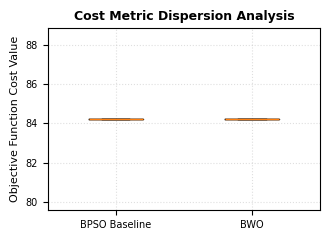
\includegraphics[width=\linewidth]{execution_results/cost_metric_dispersion_analysis_instance_small.png}
        \caption{Dispersión Instancia Pequeña}
    \end{subfigure}
    \caption{Trayectorias de convergencia y diagramas de caja para la instancia pequeña ($3 \times 5$), los cuales ilustran rutas de optimización idénticas y una convergencia perfecta hacia el óptimo global.}
    \label{fig:small_plots}
\end{figure}

Los registros visuales para la instancia pequeña (Figura~\ref{fig:small_plots}) muestran trayectorias de optimización idénticas. Ambos algoritmos convergen rápidamente hacia el óptimo matemático exacto en las iteraciones iniciales, manteniendo una varianza de cero en todas las generaciones posteriores.

\begin{figure}[H]
    \centering
    \begin{subfigure}[b]{0.49\linewidth}
        \centering
        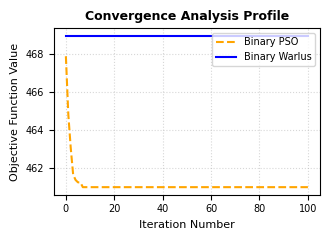
\includegraphics[width=\linewidth]{execution_results/convergence_analysis_instance_medium.png}
        \caption{Convergencia Instancia Mediana}
    \end{subfigure}
    \hfill
    \begin{subfigure}[b]{0.49\linewidth}
        \centering
        
\includegraphics[width=\linewidth]{execution_results/cost_metric_dispersion_analysis_instance_medium.png}
        \caption{Dispersión Instancia Mediana}
    \end{subfigure}
    \caption{Trayectorias de convergencia y diagramas de caja para la instancia mediana ($10 \times 25$). El algoritmo BPSO muestra estancamiento prematuro, mientras que BWO mantiene una varianza exploratoria activa.}
    \label{fig:medium_plots}
\end{figure}

Para la escala mediana (Figura~\ref{fig:medium_plots}), las curvas de convergencia evidencian la vulnerabilidad de BPSO ante el estancamiento prematuro, generando una línea plana constante en el valor de $461,0000$, lo que demuestra una pérdida total de diversidad en la población. Por el contrario, la trayectoria de BWO muestra una exploración estructural activa, exhibiendo una dispersión de soluciones más amplia a lo largo de las generaciones. 

\begin{figure}[H]
    \centering
    \begin{subfigure}[b]{0.49\linewidth}
        \centering
        
\includegraphics[width=\linewidth]{execution_results/convergence_analysis_instance_large.png}
        \caption{Convergencia Instancia Grande}
    \end{subfigure}
    \hfill
    \begin{subfigure}[b]{0.49\linewidth}
        \centering
        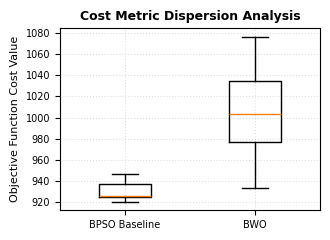
\includegraphics[width=\linewidth]{execution_results/cost_metric_dispersion_analysis_instance_large.png}
        \caption{Dispersión Instancia Grande}
    \end{subfigure}
    \caption{Trayectorias de convergencia y diagramas de caja para la instancia grande ($20 \times 50$), mostrando la explotación local efectiva de BPSO y la exploración extendida de BWO.}
    \label{fig:large_plots}
\end{figure}

En la escala grande (Figura~\ref{fig:large_plots}), las curvas de convergencia muestran que BPSO aprovecha de manera efectiva su mecánica de explotación local. Esto le permite al enjambre aproximarse de forma estable al óptimo global, logrando una distribución estrecha cerca del piso de $920,3000$. En el caso de BWO, se aprecia un proceso de búsqueda exploratorio más extendido, manteniendo una dispersión de soluciones más amplia a través del límite de $100$ iteraciones establecido.

\section{Discusión y Compensaciones Algorítmicas}
\label{sec:discussion}
Los resultados experimentales muestran una clara relación de compromiso \textit{(trade-off)} entre los mecanismos de exploración y explotación dentro de espacios discretos de ubicación y asignación. El algoritmo BPSO se apoya fuertemente en su función de transferencia sigmoidea, operando en conjunto con coeficientes fijos de aceleración cognitiva y social. Si bien esta estructura incrementa considerablemente el riesgo de convergencia prematura —como se evidenció en el estancamiento absoluto en el valor de $461,0000$ para la escala mediana—, provee una ventaja competitiva relevante en topografías de búsqueda de mayores dimensiones donde la explotación del gradiente local se vuelve crítica. En la escala grande, esta intensa búsqueda local permitió a BPSO consolidar un conjunto de soluciones significativamente más cercano al óptimo global establecido, registrando una Brecha de Optimización de apenas $+0,56\%$.

En contraste, el algoritmo BWO incorpora un conjunto más diverso de fases conductuales, utilizando transiciones de migración dinámica, conductas de protección social y el modelado de estados de combate agresivos. Esta variabilidad arquitectónica previene el colapso temprano de la población de agentes y sustenta una exploración sostenida a través de escenarios de búsqueda complejos, lo cual le permitió evadir con facilidad el mínimo local que estancó a BPSO en la escala mediana.

Sin embargo, esta alta varianza exploratoria se transforma en una desventaja operativa cuando se dispone de presupuestos iterativos restringidos dentro de espacios de alta dimensionalidad. En la escala grande, BWO dispersó su esfuerzo de búsqueda en múltiples frentes conceptuales, lo que resultó en un número insuficiente de generaciones disponibles para explotar a fondo las regiones de interés localizadas. La menor tasa de convergencia local se tradujo en una mayor dispersión final ($\sigma = 34,2454$) y en una Brecha de Optimización superior ($+1,96\%$). Estos hallazgos sugieren que el rendimiento de BWO podría optimizarse sustancialmente mediante la inclusión de una función de transferencia adaptativa o un mecanismo de enfriamiento acelerado, orientados a potenciar sus capacidades de explotación a medida que el algoritmo avanza hacia sus etapas generacionales tardías.

\section{Conclusión}
\label{sec:conclusion}
Este estudio evaluó el Problema de Localización y Asignación de Microhubs de Dos Escalones (TMLPA) comparando el Algoritmo de la Morsa Binario (BWO) contra el de Optimización por Enjambre de Partículas Binario (BPSO) bajo límites globales exactos, resueltos mediante el motor de HiGHS MILP engine. El diseño experimental utilizado integró un módulo automatizado de reparación de restricciones e implementó un protocolo dinámico de manejo de valores atípicos para garantizar la consistencia estadística.($N=30$). 

A pesar de que ambas metaheurísticas resuelven el problema a menor escala sin dificultad, los hallazgos empíricos muestran que su rendimiento diverge significativamente a medida que las dimensiones del problema escalan. BPSO demuestra una gran capacidad de explotación local a gran escala, logrando una brecha de optimización ajustada de $+0.56\%$, pero sigue siendo muy vulnerable a la convergencia prematura en topografías multimodales de escala media. Por el contrario, BWO destaca por preservar la diversidad de la población y evitar trampas locales tempranas, pero presenta tasas de explotación más lentas en espacios de búsqueda de alta dimensión. 

%------------------------------------
\bibliography{refs}
\end{document}